%recently finished my uni and get to start choosing where and what I want to do.
%spent a year in japan
%would like to experience more of the world
%want to play in an organisation that has room for growth and the opportunity to effect the way people do things
%


\documentclass[10pt, a4paper]{report}
\usepackage{geometry}                % See geometry.pdf to learn the layout options. There are lots.
\geometry{lmargin=1cm}
\geometry{rmargin=1cm}
\geometry{tmargin=1cm}
\geometry{bmargin=1cm}



\title{Curriculum Vitae}
\author{Bodey Baker}
%\date{}                                           % Activate to display a given date or no date

\parindent 0pt
\parskip 5pt
\pagestyle{empty}

%\usepackage{CJK}
\usepackage{mdwlist}
\usepackage{graphicx}
\usepackage{booktabs}
\usepackage{flafter}  % Don't place floats before their definition
\usepackage{amsmath,amssymb}  % Better maths support & more symbols
\usepackage[utf8]{inputenc} % Any characters can be typed directly from the keyboard, eg éçñ
%\usepackage{geometry} % to change the page dimensions
\usepackage{enumitem}
\usepackage{hyperref}
\setitemize{noitemsep,topsep=0pt,parsep=0pt,partopsep=0pt,leftmargin=1em}

%empty
\newcommand{\teaching}[1]{}
\newcommand{\engineering}[1]{}
\newcommand{\verbose}[1]{}

%teaching resume (needs to be 2 pages)
%\renewcommand{\teaching}[1]{#1}
%\renewcommand{\engineering}[1]{}
%\renewcommand{\verbose}[1]{}

%Engineering CV
\renewcommand{\teaching}[1]{#1}
\renewcommand{\engineering}[1]{#1}
\renewcommand{\verbose}[1]{#1}

\newcommand{\wh}[5]{{\bf{#2 \hfill #1}}
\begin{tabular}{ll}
\parbox[t]{13cm}{#5}
& \parbox[t]{5.3cm}{ \raggedleft{ {#3}\\{#4}\\}}\end{tabular}~\\~\\}

%\newcommand{\sk}[3]{\begin{basedescript}{\desclabelstyle{\pushlabel}\desclabelwidth{10em}}
%\item[#1] #2 \end{basedescript}#3}
\newcommand{\sk}[3]{\subsubsection*{#1} {#2}{#3}}

\newcommand{\pa}[3]{#1 - #2}

\makeatletter\let\MPtrue\@minipagetrue\makeatother

\title{Curriculum Vitae\\~\\of}
\author{Bodey Baker}% \\(?????????)\\ \\}



\begin{document}

\begin{minipage}{13cm}
\begin{tabular}{ll}
{\bf Name} & Bodey Royce Baker \\ 
{\bf Date of Birth} & 5th October 1984 \\
{\bf Citizenship} & Australian \\
{\bf Email} & \href{mailto:bodey.baker@gmail.com}{bodey.baker@gmail.com} \\
{\bf Phone} & +82-10-2186-1005 \\
{\bf Location} & Seoul, South Korea \\
\end{tabular}
\section*{Summary}
I am a native English speaker from Australia living in Korea and now I am hoping to get some more experience teaching for a few years. \\

Since the start of March this year I've been working for Wonderland as a homeroom teacher of the year six year and loving it. Previously I taught English in primary schools and junior high schools both following a curriculum and planning my own lessons. I have also tutored and demonstrated for engineering and programming units at the University of Western Australia as well as attending their ``Seminars, Tutorials and Laboratories" teaching course. During my time working and studying at this university I published three academic papers and presented two at conferences. One of these was during the honours research year of my Computer Science degree where I topped the unit ``Scientific Communication'', a unit concentrating on academic writing. \\

I really enjoy teaching and now I would like to expand the teaching skills and experience I currently have.
\end{minipage}
\hfill
\begin{minipage}{50mm}
{%
\setlength{\fboxsep}{0pt}%
\setlength{\fboxrule}{1pt}%
\fbox{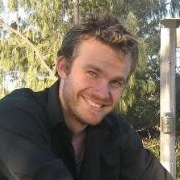
\includegraphics[height=40mm]{pic7.jpg}}%
}%
\end{minipage}
%{I have attended the "Seminars, Tutorials and Laboratories" teaching course at the University of Western Australia. Following this I tutored the units ``Modelling and Computing Analysis for Engineers" and ``Mechatronics Systems" for one semester.}
%%\sk{English Ability}{I am a native English speaker from Australia who has completed a computer science bachelors degree with honours and written three scientific papers that have been published.}
%\item[Languages] English (Native), Japanese (Basic-Intermediate), Korean (Basic)
%\item[Operating Systems] Linux, UNIX, Mac OS X, Windows XP/7
%\end{basedescript}
\section*{Experience}
\wh{March 2013 - Current}
{English Homeroom Teacher}
{Wonderland}
%{35 Stirling Hwy.\\ Crawley WA 6009\\ Australia
{Seoul, Korea}
{
\begin{itemize}
\item Planning lessons; teaching students English, art and science; and general care of kindergarten students.
\item Teaching conversation and grammar to Elementary students.
\end{itemize}
}

\wh{July 2010 - July 2012}
{Avionics Software Engineer}
{Cyber Technology}
{Australia}
{\begin{itemize}
\item Worked in a professional setting programming and designing software for UAVs.
\item Wrote internal documentation and manuals.
\end{itemize}
}

\wh{July 2009 - November 2009}
{Tutor}
{University of Western Australia}
%{35 Stirling Hwy.\\ Crawley WA 6009\\ Australia
{~}
{
\begin{itemize}
\item Tutored the units:
\begin{itemize}
\item Modelling and Computing Analysis for Engineers
\item Java
\end{itemize}
\item Required ability to explain difficult concepts to students who were struggling.
\item Duties: teaching, lab demonstrating and marking.
\end{itemize}
}

\wh{May 2009 - June 2010}
{Undergraduate Engineer}
{JRB Engineering}
%{24 Drummond Pl. \\ West Perth WA 6005\\ 
{Australia}
{
\begin{itemize}
\item Presented reports on the analysis of accelerometer data to ensure vehicles met vibration requirements.
\end{itemize}
}

\wh{May 2008 - February 2009}
{Assistant English Teacher}
{W5 Staff Services}
{Japan \\ ~}
{
\begin{itemize}
\item Taught English to primary and junior high school students.
\item Duties: planning lessons; teaching; communicating with students.
\item Skills: teaching; public speaking; motivating others; integrating into new cultures.
\end{itemize}
}

\engineering{
\wh{August 2007 - January 2008}
{Research Assistant}
{iVEC at the ARRC}
{Australia}
{
\begin{itemize}
\item Tested a method to explore the structure of a rock sample from 3D data and visualise the output using a 3D projector.
\end{itemize}}
}

\newpage

\wh{July 2007 - November 2007}
{Tutor}
{University of Western Australia}
%{35 Stirling Hwy.\\ Crawley WA 6009\\ Australia
{~}
{
\begin{itemize}
\item Tutored the units:
\begin{itemize}
\item Modelling and Computing Analysis for Engineers
\item Mechatronics Systems
\item Java
\end{itemize}
\end{itemize}
}

\wh{December 2006 - December 2007}
{Research Assistant}
{Centre for Exploration Targeting \\ University of Western Australia}
{~\\~}
{
\begin{itemize}
\item Studied how roughness changes with direction across rock surfaces.
\item Finished with a talk and poster explaining the results to the public
\item Published a paper with an academic journal
\end{itemize}
}

\section*{Education}

\subsection*{Bachelor of Engineering (Mechatronics)}
	\begin{basedescript}{\desclabelstyle{\pushlabel}\desclabelwidth{2em}}
	\item[2011:] The University of Western Australia
	\end{basedescript}
The final year project took an expensive damage detection system and modified it to use cheaper and smaller electronics. This required design, planning, mathematical analysis of sensor readings, and finally a public talk explaining the project.
\subsection*{Bachelor of Computer Science} % Honours (2A)
\begin{basedescript}{\desclabelstyle{\pushlabel}\desclabelwidth{2em}}
	\item[2006:] The University of Western Australia
	\end{basedescript}
The final year project was ``Strategy specification for teamwork in robot soccer". This project ended with a conference paper being presented in front of other researchers and students. Also, because the project used robot dogs, we often did demonstration shows entertaining children and their parents.
\section*{Scholarships and Prizes}
{\bf 2007:} Top of the Computer Science honours unit ``Scientific Communication" \newline
{\bf 2001:} \parbox[t]{32em}{Institute of Engineers award for attaining a TEE score above 75\% in:\\
Chemistry, Physics, Calculus and Applicable Mathematics.} \newline
{\bf 2000:} Olympic Torch Escort Runner	 \newline
\section*{Professional affiliations}
{\bf 2007-2008:} Webmaster of Ancestrais Capoeira \newline
{\bf 2007:} President of the UWA Association of Mechatronics Engineers \newline
{\bf 2006:} Social Engineer of the UWA Association of Mechatronics Engineers \newline
{\bf 2006:} Vice-President of the UWA Computer Science Students' Club \newline
{\bf 2005:} Ordinary Committee Member in the UWA Computer Science Students' Club \newline
% \section*{Volunteer Activities}
\section*{Interests}
Soccer, Rock Climbing, Acrobatics, Capoeira, Machine Learning, Languages, Snow Boarding, Travelling, Cultures.

%\section*{Quotations}
%{\large ``Bodey is amazing! Best housemate ever!''}
%
%~\hspace*{4em} {\bf Brent} - {\em Worst Landlord Ever}
%
%\vspace{1em}
%
%\hfill {\large ``Amazing! Always has back when I leave fish in the Freezer!''}
%
%\hfill {\bf Sarah} - {\em Token Asian Chick} \newline
%\begin{tabular}[h*]{lcr}
%\parbox{5cm}{{\bf Jim Blair}\\ Managing Director\\ JRB Engineering\\ West Perth WA\\  +61 4 1904 1710\\ JimBlair@jrbeng.com.au} &
%\parbox{5cm}{{\bf Dr Klaus Gessner}\\ Senior Lecturer\\ University of WA\\ Crawley WA\\ +61 8  6488 7148 \\ kgessner@cyllene.uwa.edu.au}&
%\parbox{5cm}{{\bf Dr Mark Reynolds}\\Associate Professor\\ University of WA\\ Crawley WA\\ +61 8 6488 2279 \\ mark@csse.uwa.edu.au}
%\end{tabular}

\pagebreak

\setlength{\topmargin}{-1.5in}
\setlength{\oddsidemargin}{-1in}

\begin{figure}[h!]
   \centering
   
\includegraphics[height=1.08\vsize]{a_deg_me.jpg} 
\end{figure}

\begin{figure}[h!]
   \centering
   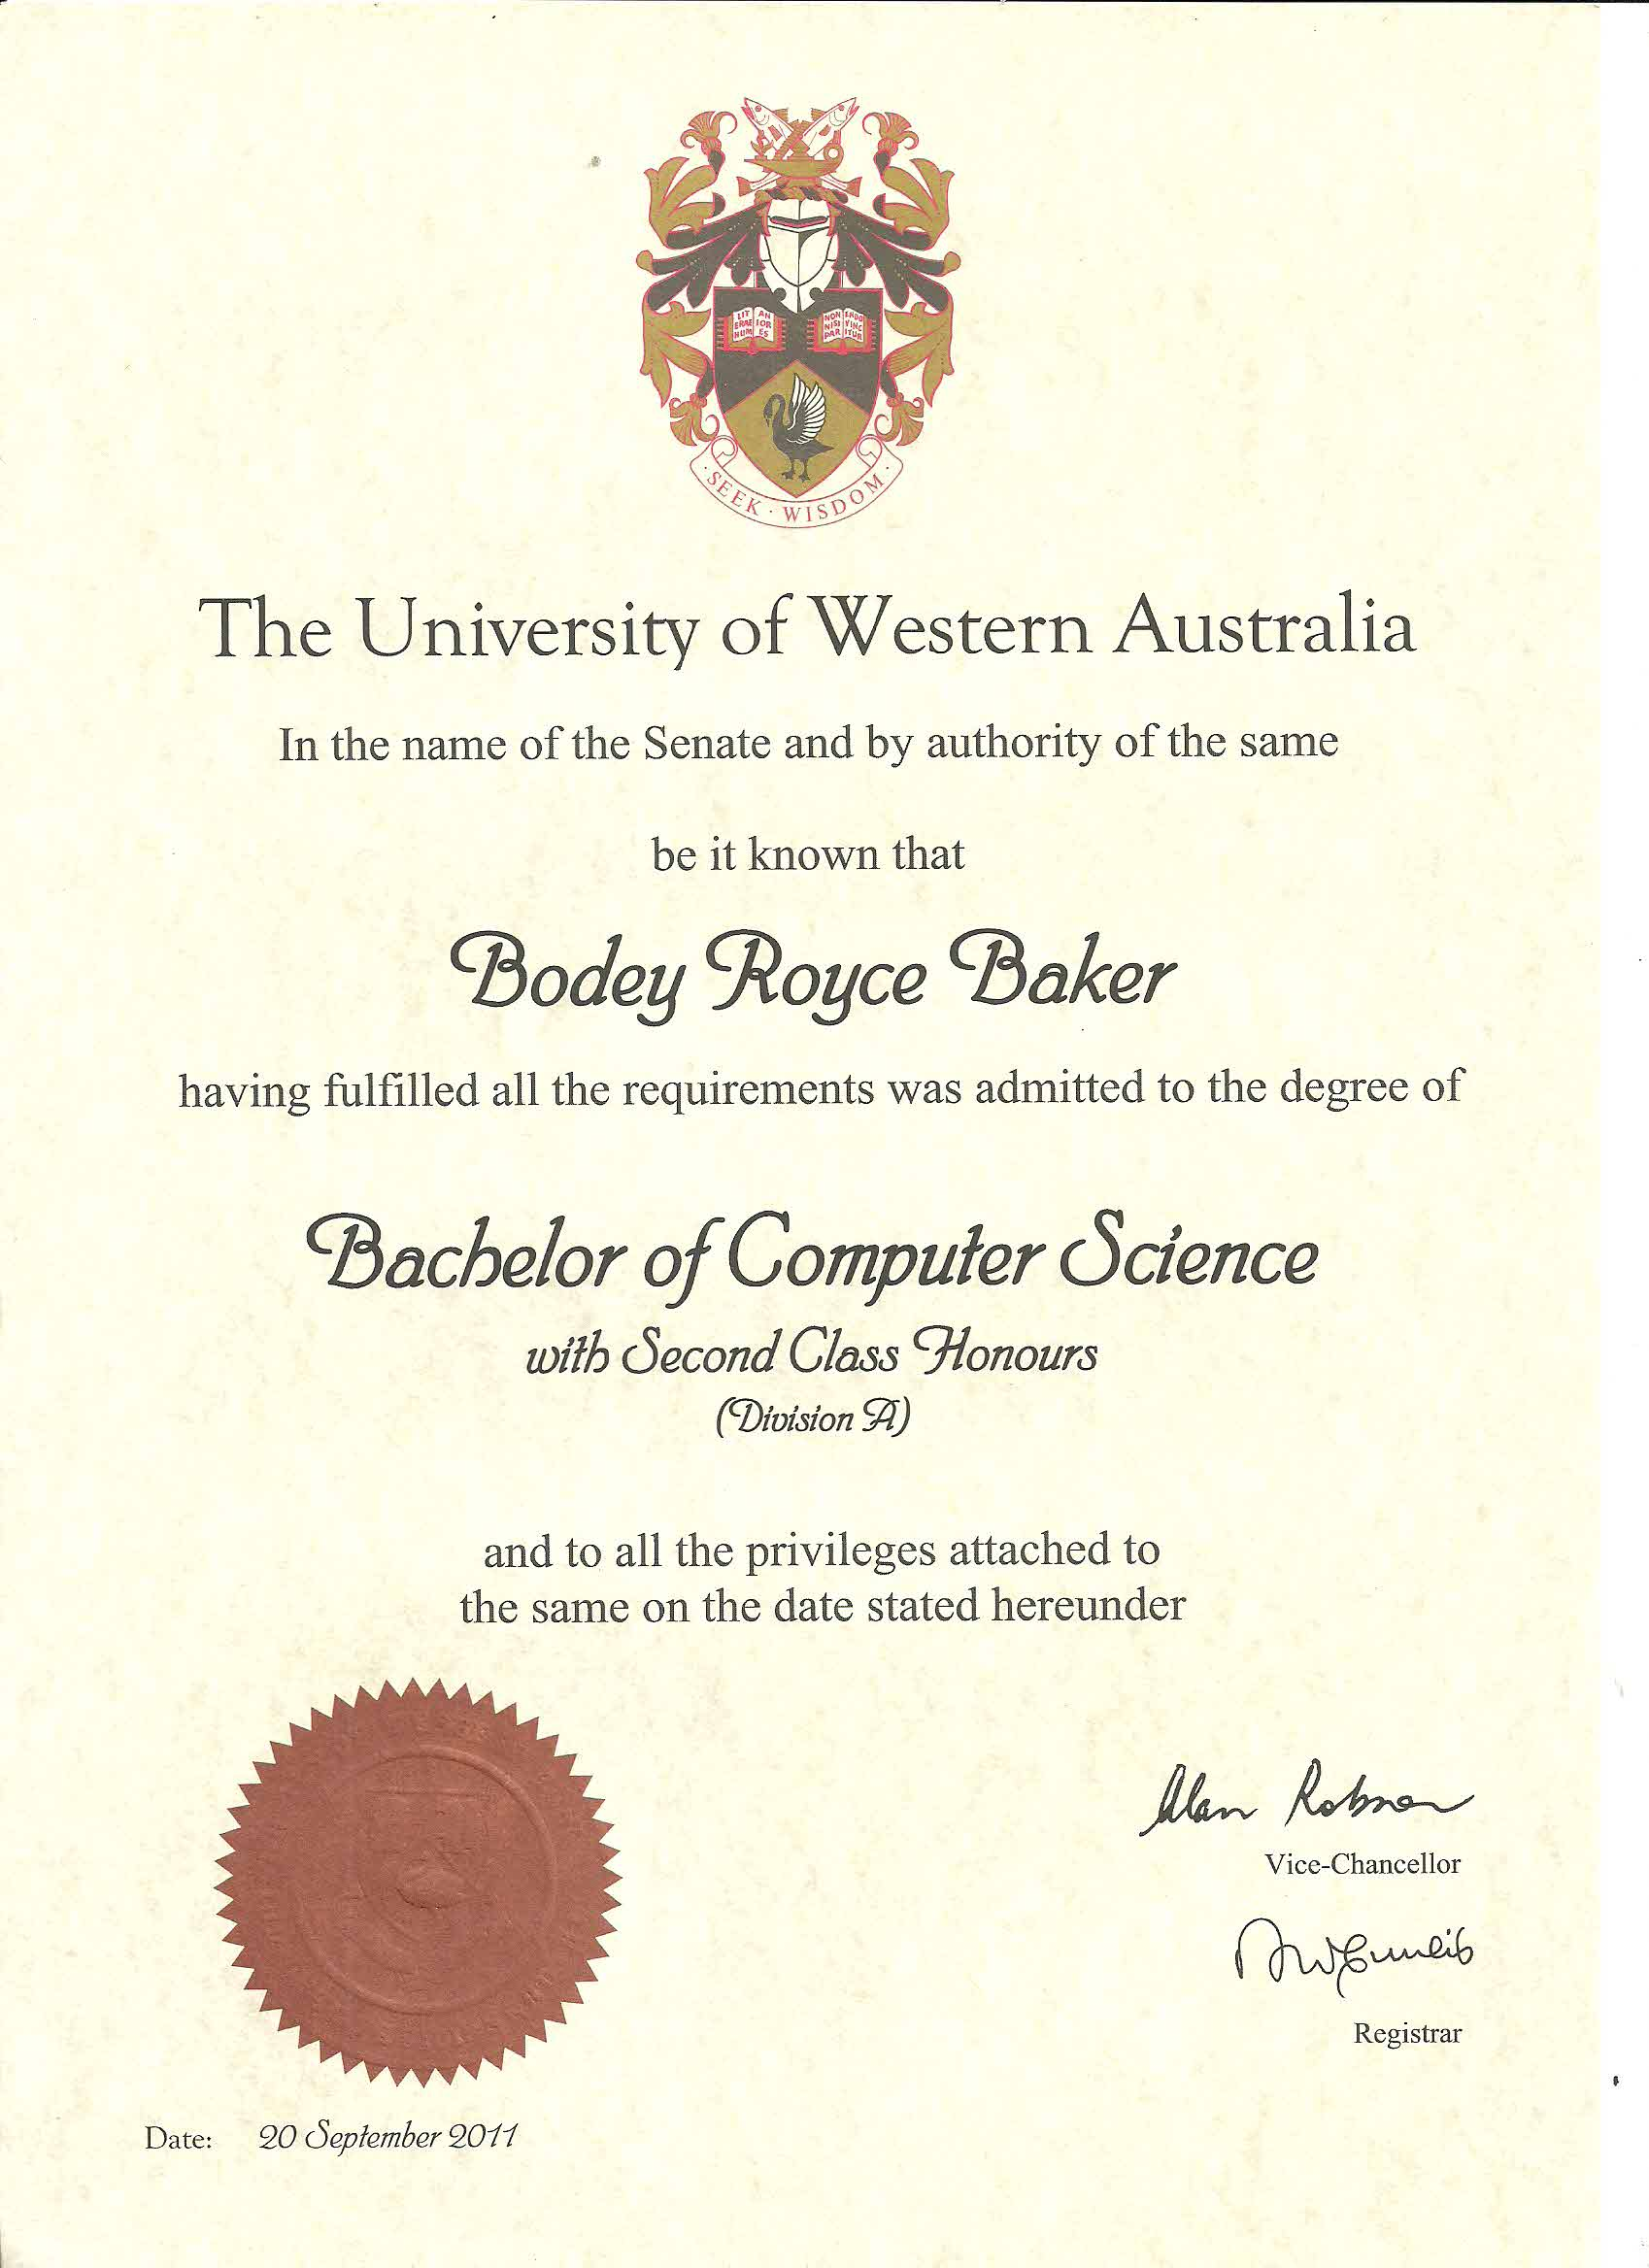
\includegraphics[height=1.08\vsize]{a_deg_cs_honours.jpg} 
\end{figure}

\begin{figure}[h!]
   \centering
   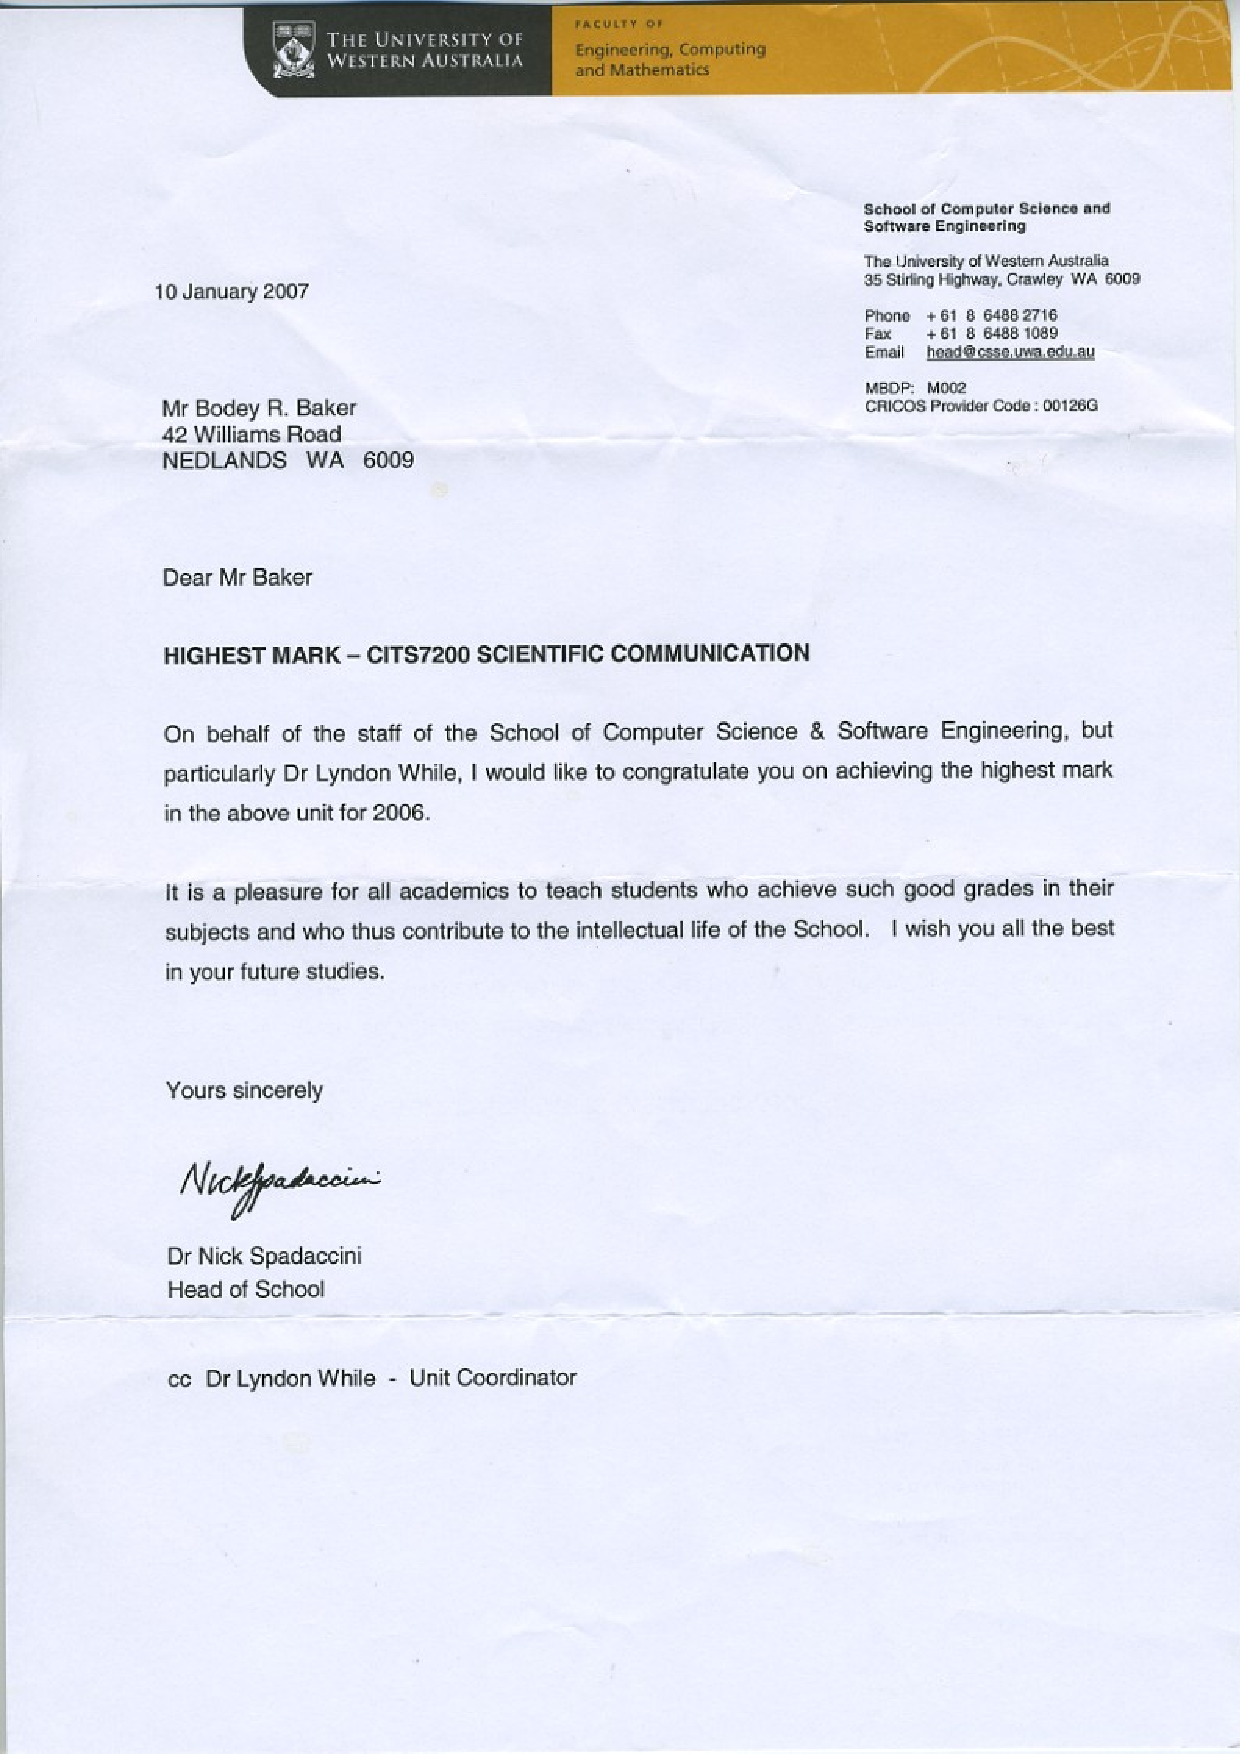
\includegraphics{a_sci_com.pdf} 
\end{figure}

\end{document}